% Created 2021-04-10 sam. 22:35
% Intended LaTeX compiler: pdflatex
\documentclass[11pt]{article}
\usepackage[utf8]{inputenc}
\usepackage[T1]{fontenc}
\usepackage{graphicx}
\usepackage{grffile}
\usepackage{longtable}
\usepackage{wrapfig}
\usepackage{rotating}
\usepackage[normalem]{ulem}
\usepackage{amsmath}
\usepackage{textcomp}
\usepackage{amssymb}
\usepackage{capt-of}
\usepackage{hyperref}
\setlength{\parindent}{0pt}
\author{Théo MEYER}
\date{2021-04-08}
\title{Explications sur mon TP3 d'IA}
\hypersetup{
 pdfauthor={Théo MEYER},
 pdftitle={Explications sur mon TP3 d'IA},
 pdfkeywords={},
 pdfsubject={},
 pdfcreator={Emacs 27.2 (Org mode 9.4.4)},
 pdflang={French}}
\begin{document}

\maketitle

\section{Minimax}
\label{sec:orgea30a24}

L'exercice demande d'appliquer l'algorithme Minimax sur l'arbre donné. J'ai recréé un arbre pour pouvoir visualiser le résultat.\\

Ci-dessous le résultat de l'application de Minimax :\\

\begin{center}
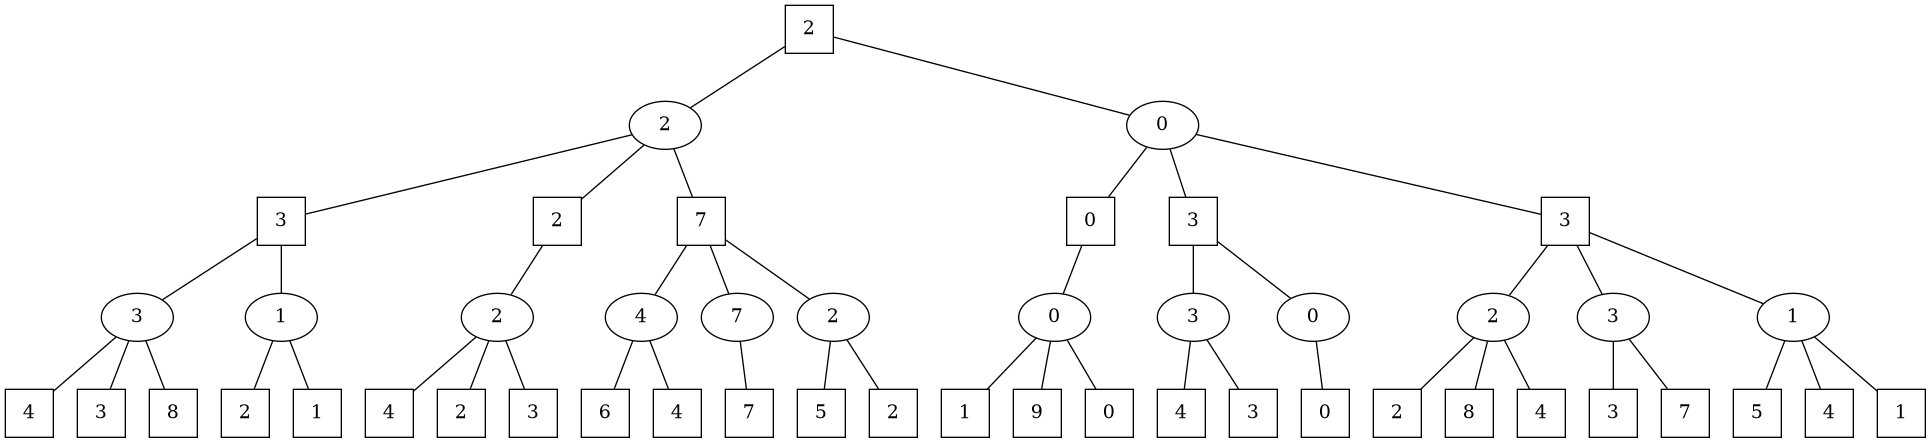
\includegraphics[width=.9\linewidth]{min_max.png}
\end{center}

La fonction récursive Minimax est appelé \textbf{48} fois, ce qui est normal puisqu'il s'agit du nombre de nœuds dans l'arbre. Minimax calcule les valeurs de tous les nœuds.\\

\pagebreak\\
\section{Élagage \(\alpha\)-\(\beta\)}
\label{sec:orgb80a71b}

Cette fois-ci, il est demandé d'appliquer l'algorithme Minimax sur l'arbre donné en utilisant un élagage \(\alpha\)-\(\beta\). Les élagages \(\alpha\) sont en bleu, et les élagages \(\beta\) sont en gris.\\

\begin{center}
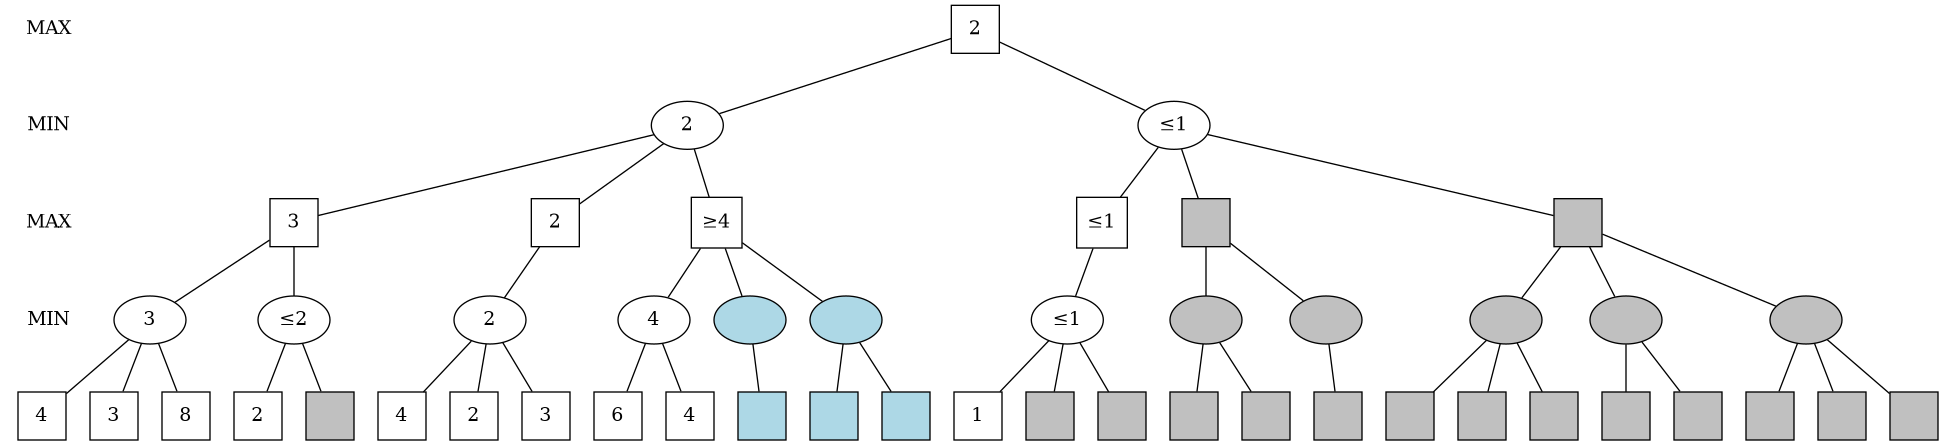
\includegraphics[width=.9\linewidth]{alpha_beta.png}
\end{center}

La fonction récursive Minimax avec \emph{élagage \(\alpha\)-\(\beta\)} est appelé \textbf{22} fois sur cet arbre, ce qui correspond à moins de la moitié du nombre d'appels par rapport au Minimax classique. (Pour information, si on commençait dans l'arbre en \emph{minimisant}, on trouve \textbf{29} appels de la fonction, ce qui est également beaucoup moins que le Minimax classique.)\\

\pagebreak\\
\section{Programmation}
\label{sec:org7fffcd1}
Pour la partie programmation, j'ai également utilisé \textbf{Clojure}, comme pour mes TPs précédents.\\

Encore une fois, \textbf{Clojure} étant un langage fonctionnel, je n'ai pas pu faire une application exacte des algorithmes donnés en cours, mais j'ai essayé de faire le plus fidèlement.\\
J'ai implémenté l'algorithme Minimax sous la version classique, et sous la version avec élagage \(\alpha\)-\(\beta\).\\

Mes deux fonctions renvoient bien la valeur \textbf{2}, qui est la valeur correcte pour l'arbre donné.\\
J'ai également prévu un moyen d'afficher le nombre d'appels récursifs à la fonction qui a été effectué, pour permettre de connaître le gain de performances en utilisant l'élagage \(\alpha\)-\(\beta\).\\

La verbosité est également choisie par l'utilisateur, s'il veut avoir une trace de l'exécution des algorithmes ou non.\\

Le code du TP est disponible sur mon compte GitHub.\\

\url{https://github.com/Tiv0w/l3-ia-tp3}\\
\end{document}
